\chapter{Implementarea sistemului}

\section{Autentificare \& autorizare}\label{4-1}
Procesul de autentificare și autorizare este realizat pe baza unui JSON web token, care este validat la accesul majorității rutelor disponibile în aplicație, excepție făcând ruta „/login”. Această logică se desfășoară în felul următor:

\begin{itemize}

	\item Dacă utilizatorul nu are un token în spațiul de stocare local și încearcă să acceseze orice pagină în afară de cea de autentificare, atunci acesta este redirecționat către pagina de autentificare și își introduce numele de utilizator și parola sa. După o autentificare cu succes a utilizatorului, acesta primește înapoi un token, ce va fi stocat în browser, pe baza căruia își va autentifica și autoriza toate cererile.

	\item Dacă utilizatorul are un token în spațiul de stocare local, acesta este trimis odată cu cererea de accesare a unei pagini și token-ul este validat, atunci utilizatorul își păstrează accesul la pagini.
	
	\item Dacă utilizatorul are un token în spațiul de stocare local, iar acesta nu este valid din diverse motive, cum ar fi faptul că acesta a expirat, faptul că token-ul a fost semnat cu o cheie ce nu se potrivește cu cea utilizată pentru verificare sau pur și simplu acesta este malformat, atunci utilizatorul este redirecționat către pagina de autentificare și este nevoit să-și introducă din nou numele de utilizator și parola pentru a primi un nou token.

\end{itemize}

În plus, aplicația utilizează o serie de coduri de răspuns HTTP pentru diferitele scenarii explicate anterior, după cum se poate observa și din figura \ref{fig:authentication}, precum 200 atunci când token-ul este valid sau 401 atunci când acesta este invalid sau credențialele sunt greșite.

\begin{figure}[H]
	\centering
	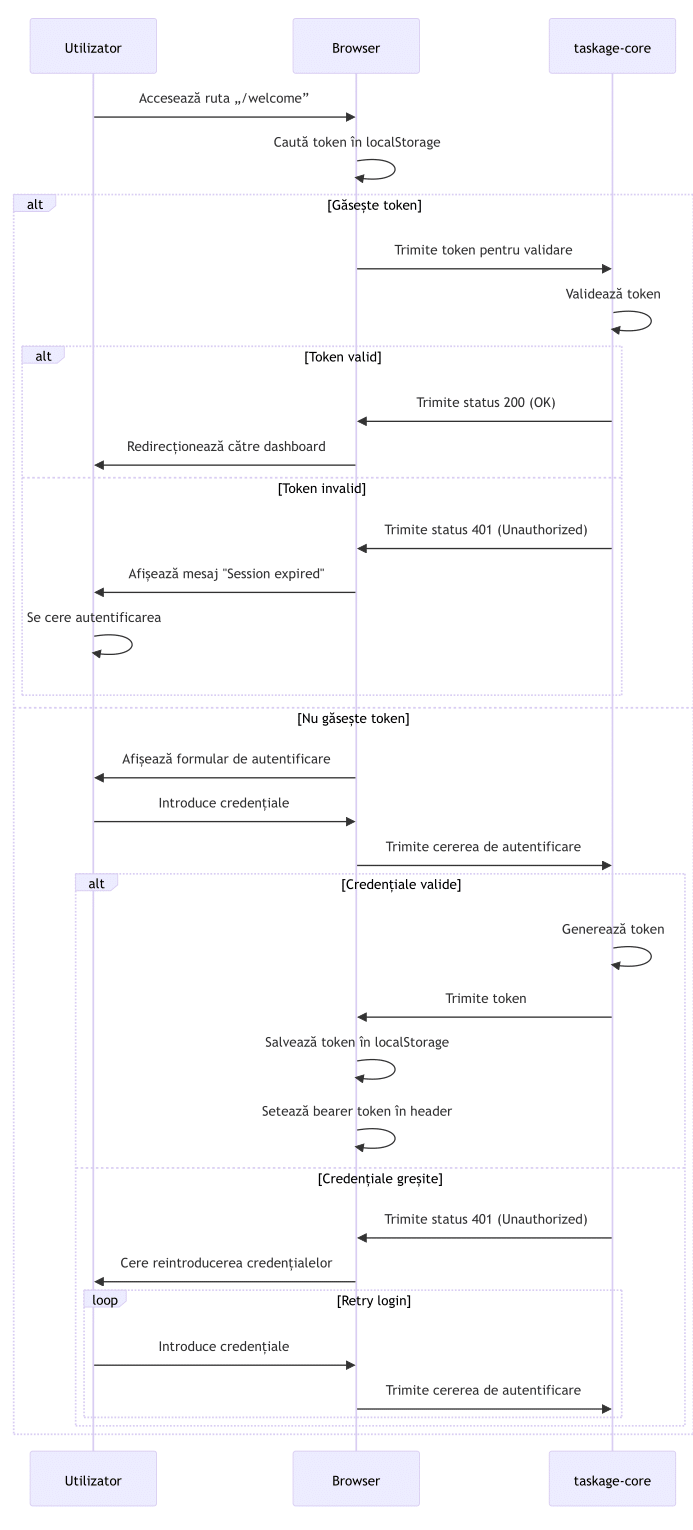
\includegraphics[width=0.6\linewidth]{seq-diagram-auth.png}
	\caption{Diagrama de secvență pentru autentificare}
	\label{fig:authentication}
\end{figure}

\section{Securitate}

Aplicația este securizată din mai multe perspective: Taskage-Client implementează o componentă personalizată de rută privată, endpoint-urile REST expuse de către componenta Taskage-Core, prin intermediul gateway-ului, sunt securizate utilizând modulul de securitate pus la dispoziție de către Spring, anume Spring Security, iar componenta Taskage-Helper este securizată prin pachetele specifice Flask.

Ruta privată a modulului front-end, utilizată în exemplul din în figura \ref{private-route-usage}, primește ca prop rolul care poate accesa ruta respectivă pentru a putea reutiliza componenta în contextul oricărui rol. Astfel, toți copiii din ierarhie, în cazul acesta rutele identificate prin constantele „TEAM_VIEW_ADMIN_LINK” și „USER_VIEW_ADMIN_LINK” vor fi protejați de logica rutei private.

\begin{figure}[H]
	\begin{lstlisting}[frame=single, style=java]
<Route element={<PrivateRoute allowedAuthRole={AUTH_ROLES.ADMIN} />} >
	<Route path={TEAM_VIEW_ADMIN_LINK} element={<TeamManager />} />
	<Route path={USER_VIEW_ADMIN_LINK} element={<EmployeeDirectory />} />
</Route>
	\end{lstlisting}
	\caption{Folosirea componentei PrivateRoute}
	\label{private-route-usage}
\end{figure}

Logica se poate observa în figura \ref{private-route}. Aceasta folosește un hook de tip „useEffect” pentru a detecta schimbarea paginii și a utilizatorului logat. Pentru oricare din aceste schimbări, încarcă un ecran de loading până verifică accesul, iar după ce metoda checkAccess determină asincron răspunsul, identifică dacă utilizatorul nu are acces la pagină fie pentru că acesta nu este logat, fie pentru că rolul său nu are dreptul pentru accesarea paginii respective. Dacă accesul este oferit, se poate încărca un „outlet”.

Outlet-ul reprezintă o componentă specifică React Router, ce ajută în dezvoltarea aplicațiilor ce implică rute imbricate. Acesta permite flexibilitatea unor componente modulare, ce pot fi incluse în cadrul aplicației, fapt dorit în cadrul aplicațiilor de tip SPA, ce ajută performanța, ridicând viteza cu care codul JavaScript este încărcat în browser-ul clientului, acesta din urmă nefiind nevoit să reîncarce toată pagina, ci doar o parte specifică. 

În cazul de față, utilizatorul este redirecționat către o pagină cu un mesaj sugestiv, după cum se poate observa în figura \ref{not-authenticated}, ce înștiințează utilizatorul cu privire la faptul ca nu este autentificat și, deci, nu are acces la conținuturile rutei accesate.

\begin{figure}[H]
	\begin{lstlisting}[frame=single, style=java]
	const PrivateRoute = observer(
	  ({ allowedAuthRole }: { allowedAuthRole: String }) => {
	    const location = useLocation();
	    const [isAllowed, setIsAllowed] = useState(false);
	    const [loading, setLoading] = useState(true);
	    const [navigateToRoute, setNavigateToRoute] = useState<string>("");
	
	    useEffect(() => {
	      const checkAccess = async () => {
	        if (userStore.currentUser) {
	          const currentUser = userStore.currentUser;
	          if (currentUser.user.authRole === allowedAuthRole) {
	            setIsAllowed(true);
	          } else {
	            setNavigateToRoute(UNAUTHORIZED_ACCESS_LINK);
	          }
	        } else {
	          setNavigateToRoute(NOT_AUTHENTICATED_LINK);
	        }
	        setLoading(false);
	      };
	
	      checkAccess();
	    }, [userStore.currentUser, location]);
	
	    return loading ? (
	      <Spin />
	    ) : isAllowed ? (
	      <Outlet />
	    ) : (
	      <Navigate to={navigateToRoute} replace />
	    );
	  }
	);
	\end{lstlisting}
	\caption{Componenta PrivateRoute}
	\label{private-route}
\end{figure}

 \begin{figure}[ht]
	\centering
 	 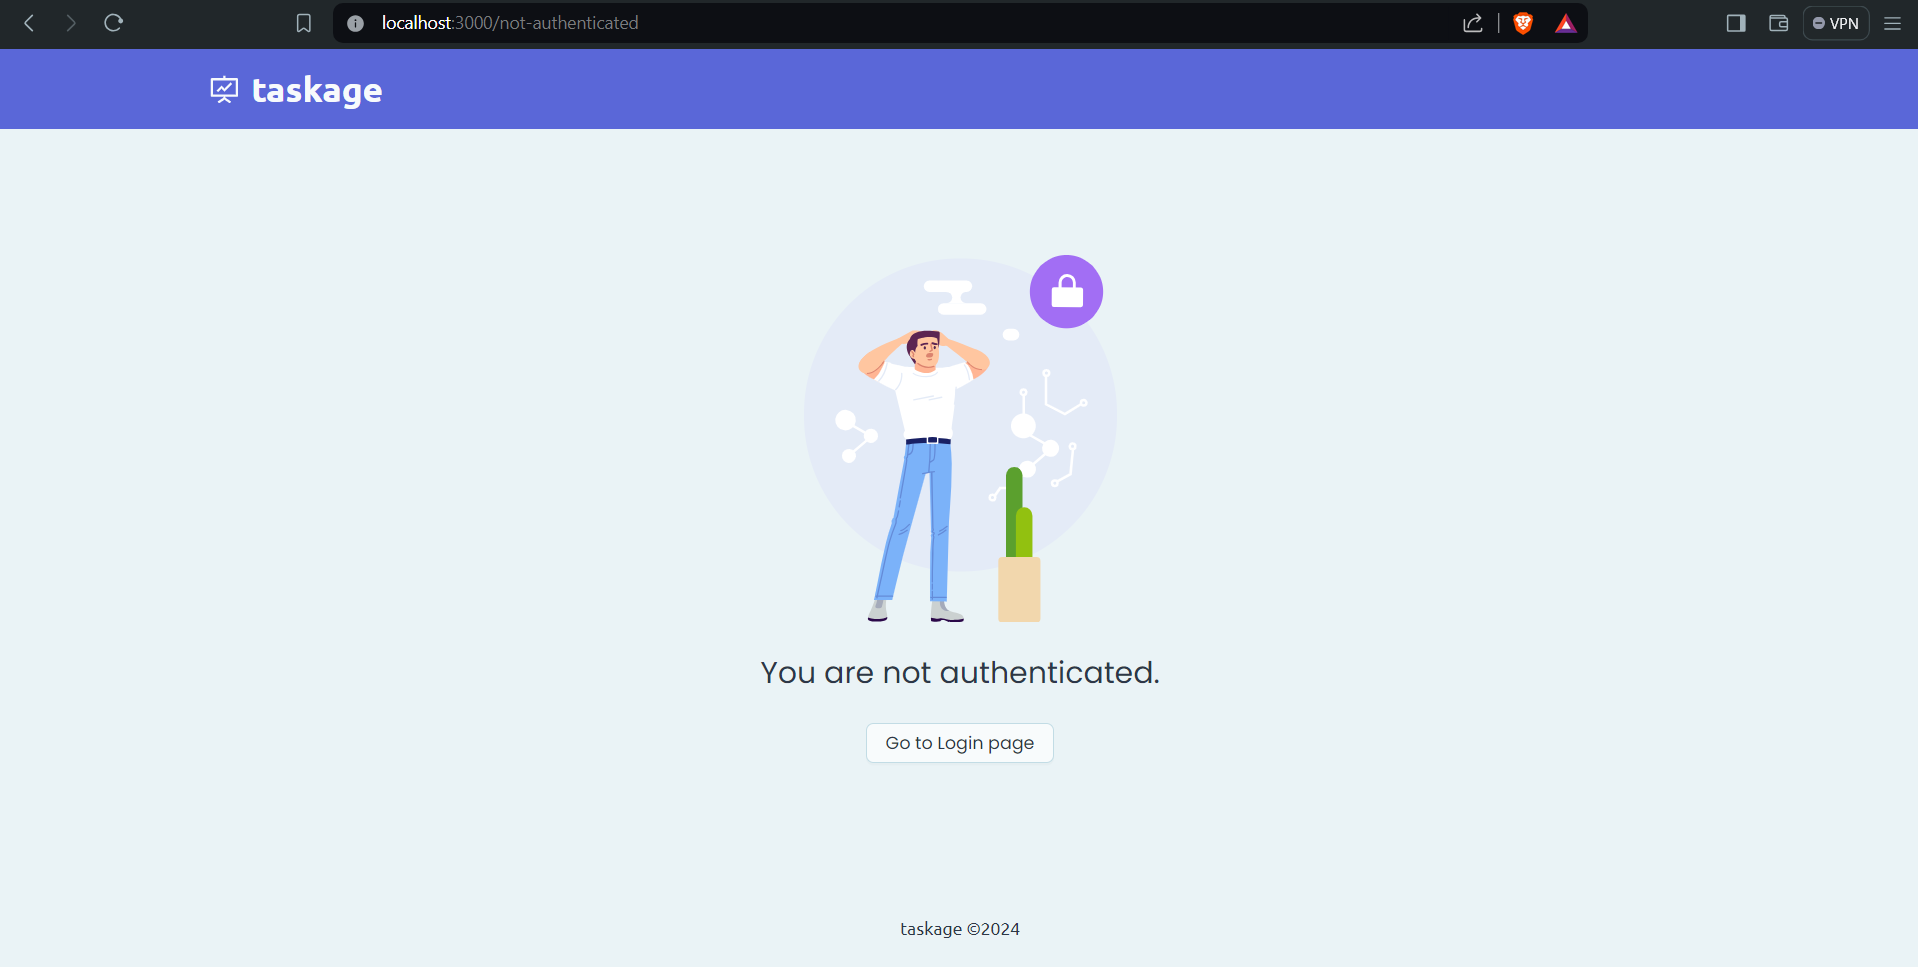
\includegraphics[width=1\linewidth]{not-authenticated.png}
	\caption{Pagina de redirecționare pentru utlilizatorii neautentificați}
	\label{not-authenticated}
 \end{figure}

Configurarea modulul Security al componentei Taskage-Core se află într-o clasa adnotată „@Configuration”, în cadrul căreia suprascriem metode precum „securityFilterChain”, „passwordEncoder” și „corsConfigurationSource”, pentru a configura gradul de securitate aplicat end-point-urilor REST. Adnotările facilitează munca dezvoltatorului, constiuind un mod de a asocia metadate diferitelor clase, pe care JVM-ul le va interpreta pentru compilare. „SecurityFilterChain” determină filtrarea securizată a cererilor pe baza token-ului, „passwordEncoder” criptează parolele înainte de salvarea în baza de date, iar „corsConfigurationService” limiteză accesul cross-origin pentru a bloca cererile care vin de pe IP-uri care nu corespund clientului nostru.

Fluxul autentificării și autorizării este definit în figura \ref{authentication-flow}. În urma conectării cu succes al unui utilizator, pe bază de nume de utilizator și parolă, componenta Taskage-Core eliberează un JSON Web Token (JWT), pe baza căruia cererile HTTP făcute ulterior de către client pot fi autorizate. Mai exact, în urma autentificării cu succes a utilizatorului se va crea un JWT, semnat de către aplicație cu ajutorul algoritmului HS512(un algoritm simetric, specific situațiilor în care cel care semnează tokenul este și cel care îl va verifica), căruia îi sunt atașate rolurile utilizatorului autentificat. Un astfel de rol este de forma „ROLE_[nume_rol]”, unde [nume_rol] poate fi orice denumire aleasă, însă, în cadrul proiectului avem trei tipuri de utilizatori: „ROLE_BASIC”(asociat membrilor normali ai unei echipe), „ROLE_MANAGER”(asociat managerilor echipelor) și „ROLE_ADMIN”(asociat administratorului paginii), fiecare având stocat în baza de date propriile privilegii și permisiuni, sub formă de roluri.

În plus, JWT-ul eliberat de către serviciul Spring are și o perioadă predefinită de existență („time to live”), configurat la compilare, iar tokenul de autorizare și datele utilizatorului curent sunt stocate în localstorage-ul browserului spre autentificarea automată. După părăsirea paginii, la o nouă accesare, se verifica dacă credențialele se află în localStorage și dacă token-ul este încă valid, print-un apel suplimentar către backend care decriptează token-ul și verifică time to live-ul setat anterior.

 \begin{figure}[H]
	\centering
 	 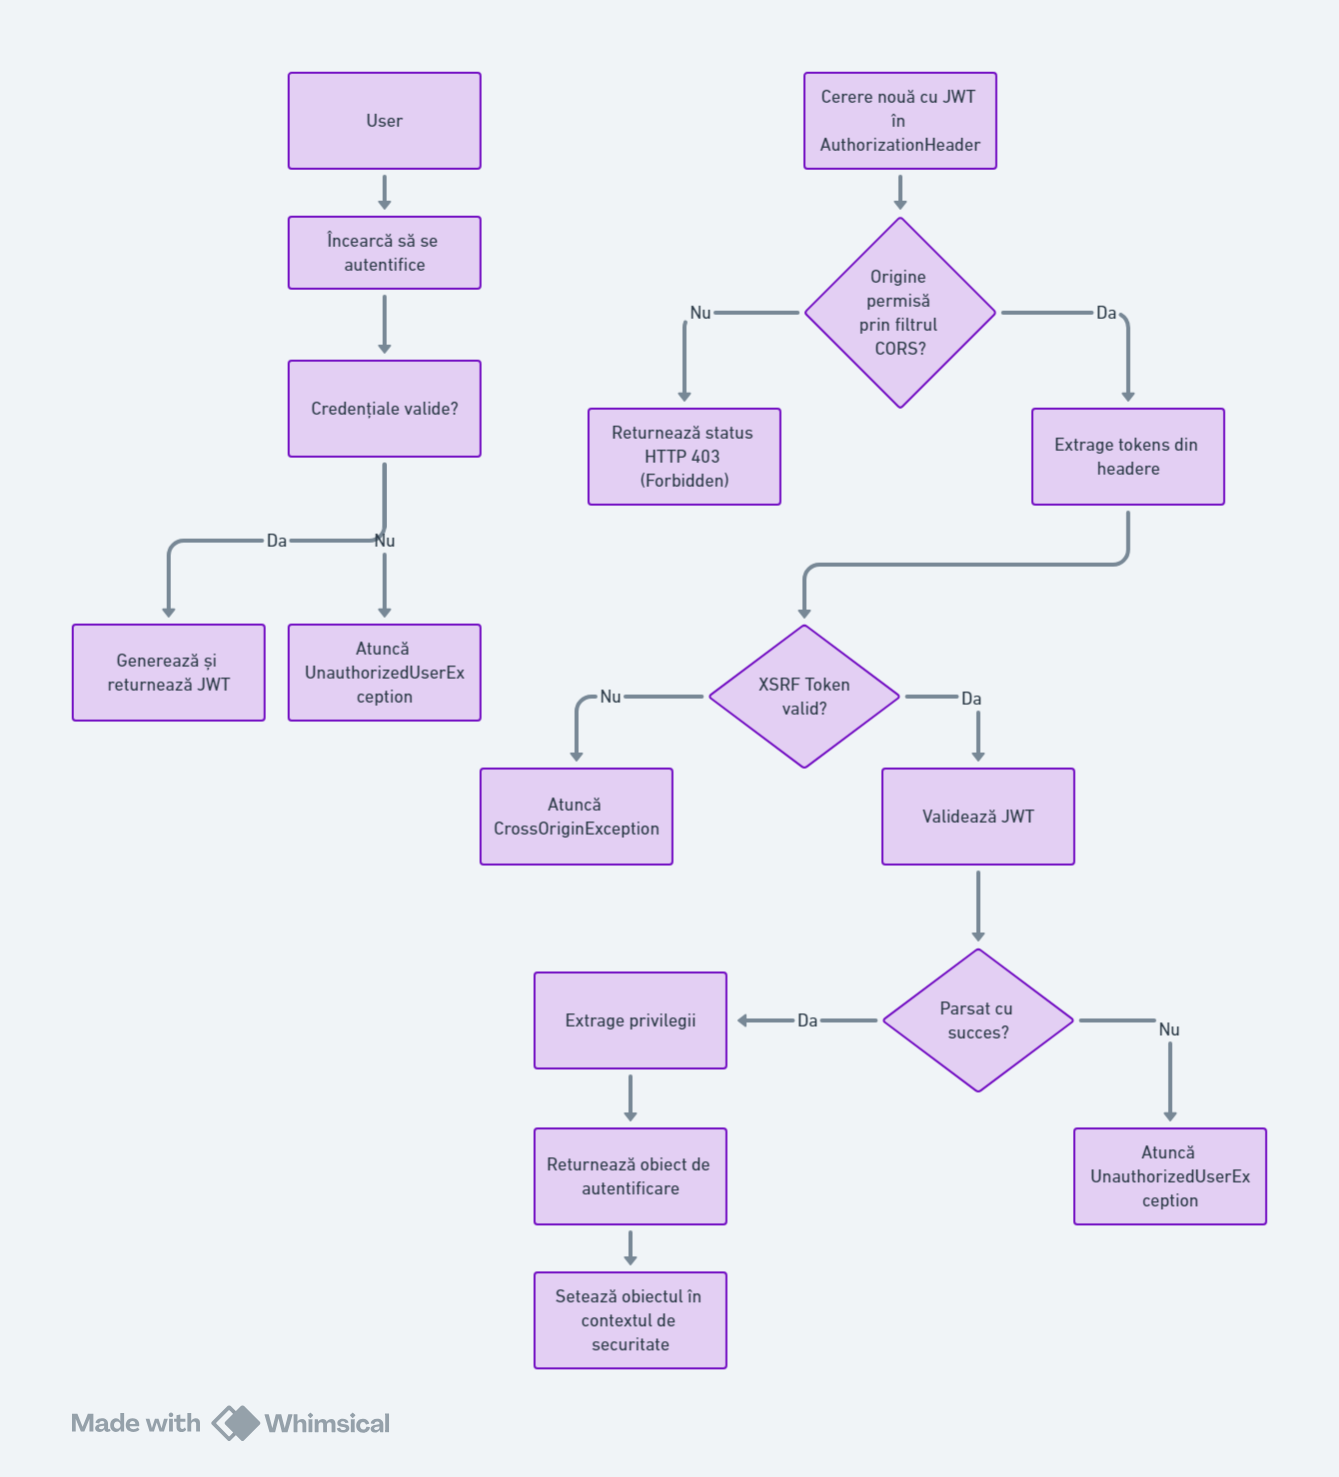
\includegraphics[width=1\linewidth]{security-flowchart.png}
	\caption{Fluxul autentificării și autorizării}
	\label{authentication-flow}
 \end{figure}

\section{Gestionarea excepțiilor}

Pentru a crește stabilitatea aplicației și a gestiona excepțiile care apar inevitabil în timpul folosirii, am implementat un strat în plus de siguranță prin crearea unei clase de gestionare a excepțiilor, care permite prinderea lor din contextul întregii aplicații și întoarcerea unui raspuns explicit clientului legat de problema întâmpinată. Pentru aceasta, am folosit adnotarea „@ControllerAdvice”, care transformă clasa într-un interceptor de excepții, pentru a fi nevoie de gestionarea excepțiilor în fiecare controller individual.

În cadrul clasei astfel definite putem explicita metoda de gestionare a fiecărei excepții care poate fi aruncată. În figura 4.6 se observă un astfel de exemplu, unde excepția este generică, dar este invocată cu un mesaj care va fi întors cu statusul explicit de către endpoint.

\begin{figure}[H]
	\begin{lstlisting}[frame=single, style=java]
@ControllerAdvice
public class GlobalExceptionHandler {
    @ExceptionHandler(NotFoundException.class)
    public ResponseEntity<String> handleNotFoundException(NotFoundException e) {
        return ResponseEntity.status(HttpStatus.NOT_FOUND).body(e.getMessage());
    }
	\end{lstlisting}
	\label{not-found-exception}
	\caption{Gestionarea excepției NotFoundException}
\end{figure}

La celălalt capăt, în componenta front-end, am identificat aceste erori și am afișat o notificare legat de problema întâmpinată. Conceptul de permisiuni din JS permite indicarea de acțiuni de executat după comanda asincronă prin metodele .then() si .catch(), așa cum apare în figura 4.7.

\begin{figure}[H]
	\begin{lstlisting}[frame=single, style=java]
create = (newTask: Task, teamId: number) => {
  axios
    .post(`${TASKS_API_URL}/create`, newTask)
    .then(() => {
      sprintStore.getAllForTeam(teamId);
      message.success("Task added successfully");
    })
    .catch((err: AxiosError) => {
      handleAxiosError(err);
      });
  };
	\end{lstlisting}
	\label{http-status}
	\caption{Gestionarea statusurilor HTTP în client }
\end{figure}


\section{Persistență}

Atât crearea schemei bazei de date, cât și interacțiunea cu baza de date, s-au realizat prin ORM-ul (Object Relational Mapping) oferit de Spring, anume Spring JPA (Jakarta Persistence API). Am optat pentru această opțiune prin configurarea specifică Hibernate, unde ddl-auto poate fi setat pentru transformarea automată a modelelor adnontate „@Entity” în scripturi SQL.

În zona de back-end, Spring JPA oferă un nivel de abstractizare peste stratul de SQL, permițând crearea de tabele, relații și constrângeri prin adnotări, precum „@Entity” pentru a semnala că această clasă reprezintă de fapt un model pentru tabela din baza de date, „@Id” pentru a semnala că un câmp dintr-o clasă asociată unei tabele este cheie primară și altele asemenea. Spring JPA ne oferă posibilitatea de a seta algoritm de generare automată a cheilor primare, de a crea coloane read-only, de a adăuga constrângeri atât banale, precum nullable și unique, cât și constrângeri relaționale precum „@OneToMany”. Codul SQL în dialectul specific, în cazul acesta PostgreSQL, poate fi vizualizat după inițializarea bazei de date:

\begin{figure}[H]
	\begin{lstlisting}[frame=single, style=yaml]
-- auto-generated definition
create table tasks
(
    assignee_id   integer
        constraint fkrwm5ssj09it2xfnlobqo3fk9x
            references app_users,
    effort_points integer,
    estimation    integer,
    id            serial
        primary key,
    priority_id   integer,
    progress      integer,
    sprint_id     integer
        constraint fkl5ac6kwptw5o73haren9qnkav
            references sprints,
    status_id     integer,
    task_type_id  integer
        constraint fkkb5gyrxp5x7p5inusg3ykdugt
            references task_types,
    description   varchar(255),
    title         varchar(255)
);

alter table tasks
    owner to postgres;
	\end{lstlisting}
	\label{http-status}
	\caption{ Cod PostgreSQL auto-generat }
\end{figure}

Un alt avantaj este specificarea metodei de aducere a datelor, care poate fi LAZY sau EAGER. În varianta LAZY, datele date de relațiile obiectului nu sunt încărcate decât la apelarea unui getter, în schimb ce varianta EAGER recuperează din start toate datele. Având în vedere că lucrăm cu o aplicație web, de ajutor mai este adnotarea „@JsonIgnore” care ne permite să manipulăm forma obiectului trimis prin HTTP. Aceasta este de multe ori necesară, pentru că reprezentarea relațiilor nu se face prin chei externe, ci prin referințe la obiectele care se află în relație, iar trimiterea acestora ca răspuns HTTP poate genera referințe circulare.

Mai departe, interacțiunea cu baza de date este simplificată, fiind mai prietenoasă cu utilizatorul decât standardul Java. În varianta standard, se folosește clasa JDBCTemplate, prin intermediul căreia ai scrie SQL nativ. În schimb, utilzând JPA, procesul este vast simplificat, având ca premise doar crearea unei interfețe ce derivează una deja existentă, generică, anume JpaRepository<TIP, TIP_ID>. 

În cadrul acestei metode, Spring JPA permite definirea de metode doar descriind acțiunea necesară. Spre exemplu, pentru a găsi toți utilizatorii dintr-o echipă anume, am putea specifica o metodă cu o signatură precum: „findAllByTeam(String)”, iar implementarea ar fi rezolvată de către ORM-ul utilizat, astfel, oferind una dintre cele mai prietenoase API-uri pentru a interacționa cu baza de date.

\section{Actualizări în timp real}

Actualizările în timp real sunt asigurate prin WebSockets. Aceștia sunt canale bidirecționale de comunicare, care funcționează pe baza unei conexiuni stabilite printr-un handshake între client și server. Într-o conexiune HTTP clasică, sunt necesare cereri repetate din partea clientului pentru a primi date de la server. Problemele cauzate sunt clare: server-ul este obligat să deschidă numeroase conexiuni TCP pentru fiecare client(unul pentru primirea datelor și unul pentru transmiterea datelor), iar clientul este forțat să țină scorul cererilor și conexiunilor pentru a corela răspunsurile.  Aceste probleme sunt rezolvate prin WebSockets, prin care cele două componente își pot trimite date fără aceste constrângeri. Din acest motiv, WebSockets sunt de ajutor pentru actualizările în timp real, fiind folosiți în aplicații precum aplicațiile de mesagerie sau jocurile multiplayer\cite{websockets-protocol}.

Pentru implementare am folosit clasicul WebSocket pus la dispoziție de JavaScript, creând clasa WebSocketService pentru gestionarea ciclului de viata a fiecărui socket, unde sunt definite event handler-ele pentru deschiderea conexiunii, primirea mesajelor și închiderea conexiunii. Am utilizat acest serviciu în cadrul store-urilor MobX, precum se poate observa în exemplul din figura \ref{websocket-reaction}. Aici am definit un reaction, concept specific MobX, ce funcționează ca un listener ce așteaptă modificarea valorii returnate de o metodă și declanșează o altă metodă ca răspuns. În acest caz, am vrut ca la autentificarea si log out-ul unui utilizator să se deschidă, respectiv închidă conexiunea, dar la deschidere să definim acțiunile și modul lor de gestionare.

\begin{figure}[H]
	\begin{lstlisting}[frame=single, style=java]
  constructor() {
	//...
    reaction(
      () => userStore.isSignedIn,
      (isLoggedIn) => {
        if (isLoggedIn) { this.connectWebSocket(); }
        else { this.disconnectWebSocket(); } }
    ); } }

  connectWebSocket = () => {
    WebSocketService.connect();
    WebSocketService.on("ADD", this.handleWebSocketMessage);
    // ... idem pentru update și delete };

  disconnectWebSocket = () => {
    WebSocketService.disconnect();
    WebSocketService.off("ADD");
    // ... idem pentru update și delete };

  updateTeamsFromWebSocket = (message: any) => {
    const { action, newTeam, teamId } = message;
    switch (action) {
      case "ADD":
        this.allTeams = this.allTeams.concat(newTeam);
        break;
      case "UPDATE":
        this.allTeams = this.allTeams.map((team) => (team.id === newTeam.id ? newTeam : team));
        break;
      case "DELETE":
        this.allTeams = this.allTeams.filter((team) => team.id !== teamId);
        break;
      default:
        break;
    } };

  handleWebSocketMessage = (message: any) => {
    this.updateTeamsFromWebSocket(message); };
	\end{lstlisting}
	\label{websocket-reaction}
	\caption{ Integrarea serviciului WebSocketService în TeamStore }
\end{figure}

Pe partea serverului, am folosit WebSockets puși la dispoziție de Spring. Aceasta a necesitat definirea unor handlers și înregistrarea lor pe diferitele rute pe care se va stabili conexiunea. Acești handleri au fost folosiți în servicii pentru ca, după efectuarea operațiilor cerute, informația nouă să fie propagată către toate sesiunile deschise.

\section{Algoritm de analiză al datelor}

Componenta Taskage-Helper are ca unic rol prelucrarea datelor stocate referitor la sarcinile de lucru. Am identificat 3 informații importante referitoare la taskuri: punctele de efort hotărâte de echipă, ce indică complexitatea, prioritatea, ce indică cât de urgentă este rezolvarea sa, și tipul, ce indică domeniul de cunoștințe folositor la indeplinirea lui(arbitrare, fiecare echipă își poate stabili propriile categorii de taskuri).

Am creat un API care primește aceste trei informații referitoare la un task și id-ul echipei în cadrul căreia e adăugat și caută să găsească persoana cea mai potrivită pentru a îl duce la capăt. O astfel de persoană este, probabil, o persoană care a mai realizat taskuri asemănătoare, iar dacă aceste taskuri sunt uzuale în echipă, membrul pentru care taskurile de acest gen sunt principale. Totuși, cele trei informații aflate la dispoziție sunt destul de diferite. Primele două sunt scalare, reprezintă metrici de evaluare ori a priorității, ori a dificultății, măsurate la rândul lor pe scări diferite, iar ultima informație, tipul de task, este o simplă etichetă reprezentată arbitrar printr-un număr. Toate acestea indică faptul că ele ar trebui tratate diferit.

Algoritmul aduce din baza de date toate informațiile curente despre taskuri realizate de echipa în cauză și calculează câte un scor de familiaritate pentru fiecare membru al echipei. Scorul este calculat ca media similarității dintre fiecare task realizat de acesta și task-ul nou, iar membrul cel mai potrivit va fi cel care a realizat, per total, cele mai similare task-uri, urmând să se țină cont și de capacitatea sa în sprintul curent.

Am menționat că două dintre detaliile referitoare la task vor fi tratate diferit de ultimul, pe baza faptului că însemnătatea este altfel interpretată. Astfel, am ales ca metode de calcul similaritatea cosinuisoidală și coeficientul Jaccard de similaritate.

Datele sunt întoarse din baza de date în tupluri de assignee_id și detalii despre task, sub forma unui array format din priority_id, effort_points și task_type_id. Primele două, având în vedere descrierea anterioară, sunt tratate separat și sunt inițial normalizate folosind MinMaxScaler din biblioteca scikit-learn. Acesta încadrează valorile uniform în intervalul [0, 1] pentru a asigura faptul că nicio caracteristică nu o să influențeze mai mult decât celelalte rezultatul.

Similaritatea cosinusoidală măsoară cosinusul unghiului dintre doi vectori, pe baza formulei: 

\[
\text{cosine_similarity} = \frac{A \cdot B}{\|A\| \|B\|}
\]

unde numărătorul este produsul scalar al vectorilor, iar numitorul este dat de produsul lungimilor vectorilor. Prin această împărțire, produsul scalar este normalizat, iar similaritatea este calculată strict pe baza direcției. Aceasta este de folos într-un context în care valorile pot varia considerabil, având în vedere că o sarcină de lucru ce necesită mult efort dar nu are prioritate mare poate să fie similară unei alte sarcini de lucru cu valori diferite, dar direct proporționale.

Coeficientul de similaritate Jaccard este folosit pentru a compara atribute categorice(etichete) și este definit ca raportul dintre cardinalul întersecției și cardinalul reuniunii a două mulțimi, rezultând formula:

\[
\text{jaccard_similarity} = \frac{|A \cap B|}{|A \cup B|}
\]


Acest coeficient măsoară similaritatea în termeni de elemente comune și este, uzual, folosită pentru date non-numerice. În cazul nostru, etichetele ce indică tipul taskurilor(de exemplu „Development” sau „Testing”) nu au o ordine naturală, deci nu putem măsura distanțe. Astfel, coeficientul Jaccard caută prezența sau absența elementelor, mai degrabă decât valorile lor. În plus, este ușor adaptabil cazurilor în care o nouă categorie este introdusă, nefiind nevoie de readaptarea algoritmului.